\documentclass{article}

\usepackage{graphicx}
\usepackage{float}
\usepackage{amsmath}
\usepackage{booktabs}
\usepackage{fullpage}
\usepackage{bm}
\usepackage{amssymb}
\usepackage[T1]{fontenc}
\usepackage{beramono}
\usepackage{listings}
\usepackage[usenames,dvipsnames]{xcolor}

%%
%% Julia definition (c) 2014 Jubobs
%%
\lstdefinelanguage{Julia}%
  {morekeywords={abstract,break,case,catch,const,continue,do,else,elseif,%
      end,export,false,for,function,immutable,import,importall,if,in,%
      macro,module,otherwise,quote,return,switch,true,try,type,typealias,%
      using,while},%
   sensitive=true,%
   alsoother={$},%
   morecomment=[l]\#,%
   morecomment=[n]{\#=}{=\#},%
   morestring=[s]{"}{"},%
   morestring=[m]{'}{'},%
}[keywords,comments,strings]%

\lstset{%
    language         = Julia,
    basicstyle       = \ttfamily\small,
    keywordstyle     = \bfseries\color{blue},
    stringstyle      = \color{magenta},
    commentstyle     = \color{ForestGreen},
    showstringspaces = false,
    aboveskip={0.9\baselineskip},
    belowskip={0.9\baselineskip},
    columns=fixed,
    extendedchars=true,
    frame=lines,
}



\author{Joris van Vugt, s4279859}
\date{\today}
\title{Statistical Machine Learning: Asssignment 3}

\begin{document}
\maketitle
\emph{Code snippets are in Julia}
\section*{Exercise 1 -- Bayesian linear regression}
\begin{enumerate}
\item The predictive distrubtion after observing these two data points is
$$ p(t| x, \bm{x}, \bm{t}) = \mathcal{N}(t|m(x), s^2(x)). $$
Using

\begin{align*}
\bm{S}_N^{-1} &= \begin{pmatrix}\alpha & 0 \\ 0 & \alpha\end{pmatrix} + N\beta\begin{pmatrix}1 & \bar{\mu}_x \\ \bar{\mu}_x & \bar{\mu}_{xx}\end{pmatrix} \\
&= \begin{pmatrix}2 & 0 \\ 0 & 2\end{pmatrix} + 20\begin{pmatrix}1 & 0.5 \\ 0.5 & 0.26\end{pmatrix} \\
&= \begin{pmatrix}22 & 10 \\ 10 & 7.2\end{pmatrix}
\end{align*}

the mean and standard deviation of the predictive distribution for each $x$ are given by

\begin{align*}
m(x) &= N\beta\begin{pmatrix}1 & x\end{pmatrix} \bm{S}_N\begin{pmatrix} \bar{\mu}_t \\ \bar{\mu}_{xt} \end{pmatrix}
\end{align*}

\begin{align*}
s^2(x) &= \beta^{-1} + \begin{pmatrix}1 & x\end{pmatrix}\bm{S}_N\begin{pmatrix} 1 \\ x \end{pmatrix}
\end{align*}

\item Using the formulas listed above, we can come up with the following code
\begin{lstlisting}
function calc_pred_dist(x, xs, t, alpha, beta)
    N = length(xs)
    S_N = ([alpha 0; 0 alpha] + N*beta*[1 mean(xs); mean(xs) mean(xs .* xs)])^-1
    mx = N*beta*[1 x]*S_N*[mean(t); mean(xs.*t);]
    s2x = beta^-1 + [1 x]*S_N*[1; x]
    mx[1], s2x[1]
end
\end{lstlisting}
See Figure \ref{fig:blr}. The main difference with Figure 3.8 from Bishop is the shape of the area of the standard deviation. This is due to the choice in basis functions. In Bishop, gaussian basis functions were used, in contrast with the constant and linear basis functions used here.

\item The probability distribution over the weights is given by
\begin{align*}
p(\bm{w}|\bm{t}, \bm{x}) &= \mathcal{N}(\bm{w}|\bm{m}_N, \bm{S}_N) \\
\bm{m}_N &= \beta\bm{S}_N\bm{\phi}^T\bm{t}=N\beta\bm{S}_N\begin{pmatrix}\bar{\mu}_t \\ \bar{\mu}_xt\end{pmatrix}
\end{align*}
and can be translated to the following procedure.
\begin{lstlisting}
function p_w(x, t, alpha, beta)
    N = length(x)
    S = ([alpha 0; 0 alpha] + N*beta*[1 mean(x); mean(x) mean(x.*x)])^-1
    m = N*beta*S*[mean(t); mean(x.*t)]
    m, S
end
\end{lstlisting}
\begin{figure}[H]
\centering
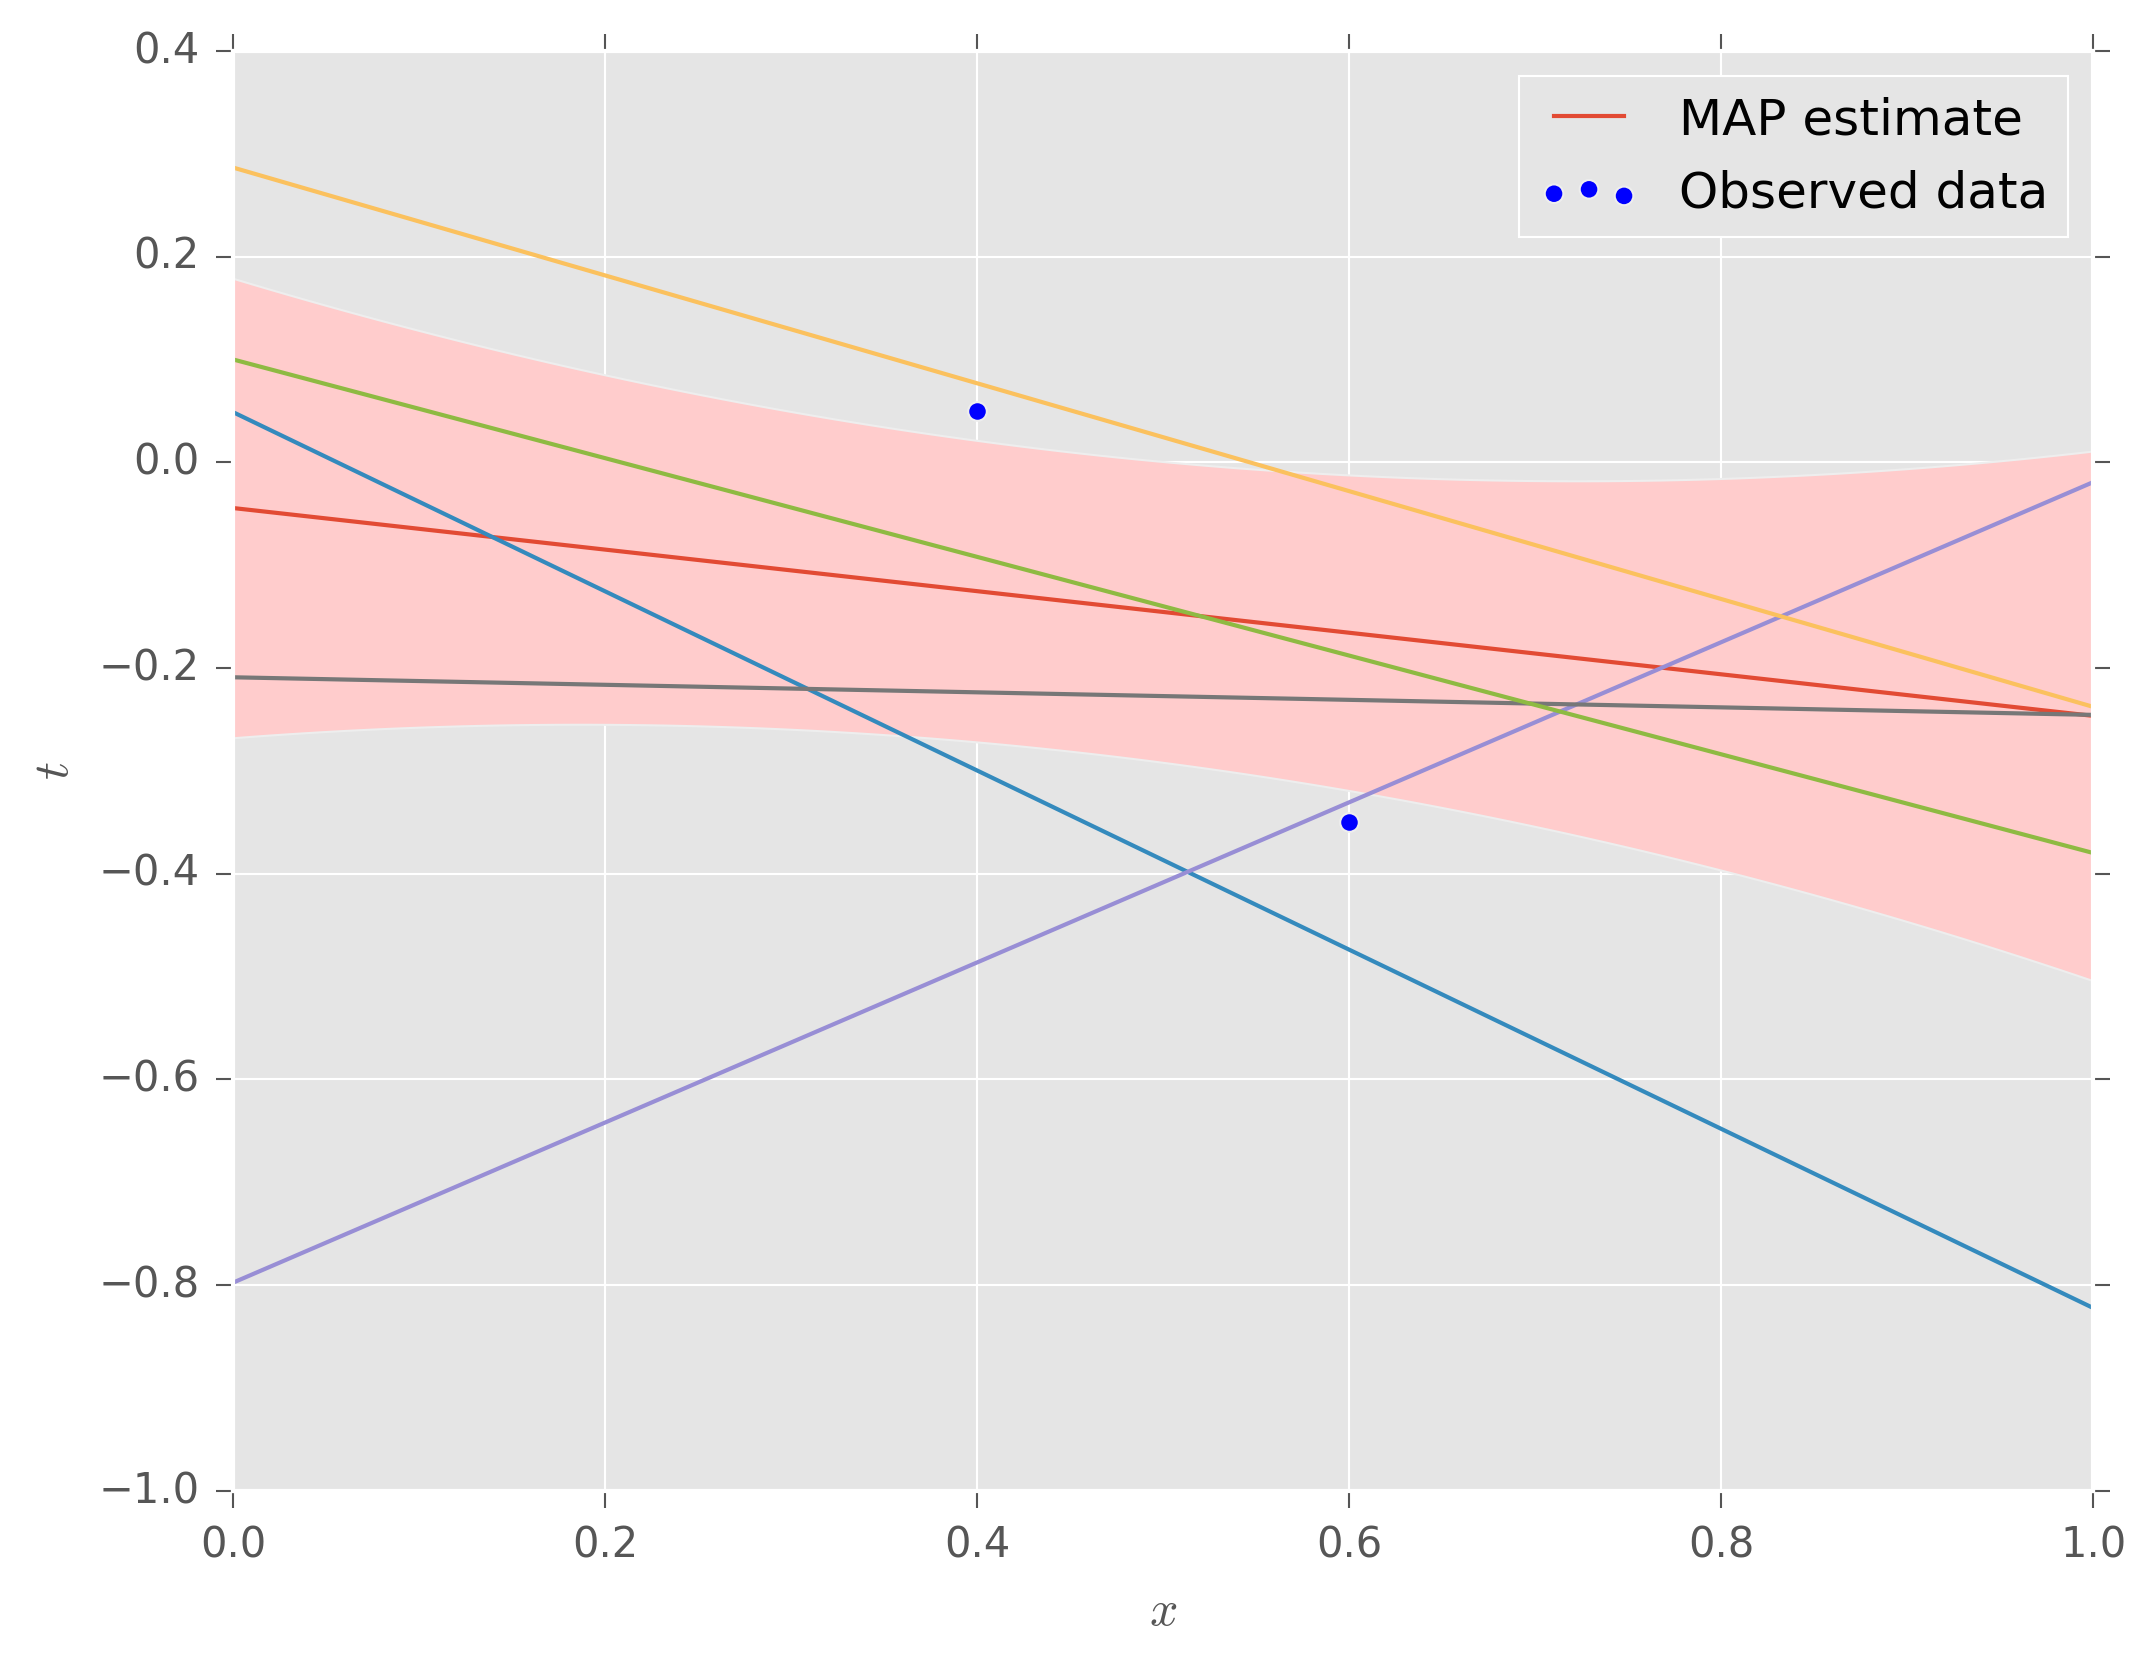
\includegraphics[width=.6\linewidth]{images/blr.png}
\caption{The blue points indicate the observed data points. The red line is the mean of the predictive distribution (i.e. the MAP estimate). The pink area indicates one standard deviation above and below the mean. The 5 other lines are functions sampled according to $p(\bm{w}|\bm{t}, \bm{x})$. See Figure \ref{fig:pw}}
\label{fig:blr}
\end{figure}
Functions can be sampled with the following code
\begin{lstlisting}
function f(x, w)
    [1 x] * w
end

m_N, S_N = p_w(x, t, alpha, beta)
weights_dist = MvNormal(m_N, S_N)
for _ in 1:5
    w = rand(weights_dist)
    y = [f(v, w) for v in vs]
    plot(vs, y)
end
\end{lstlisting}
\begin{figure}[H]
\centering
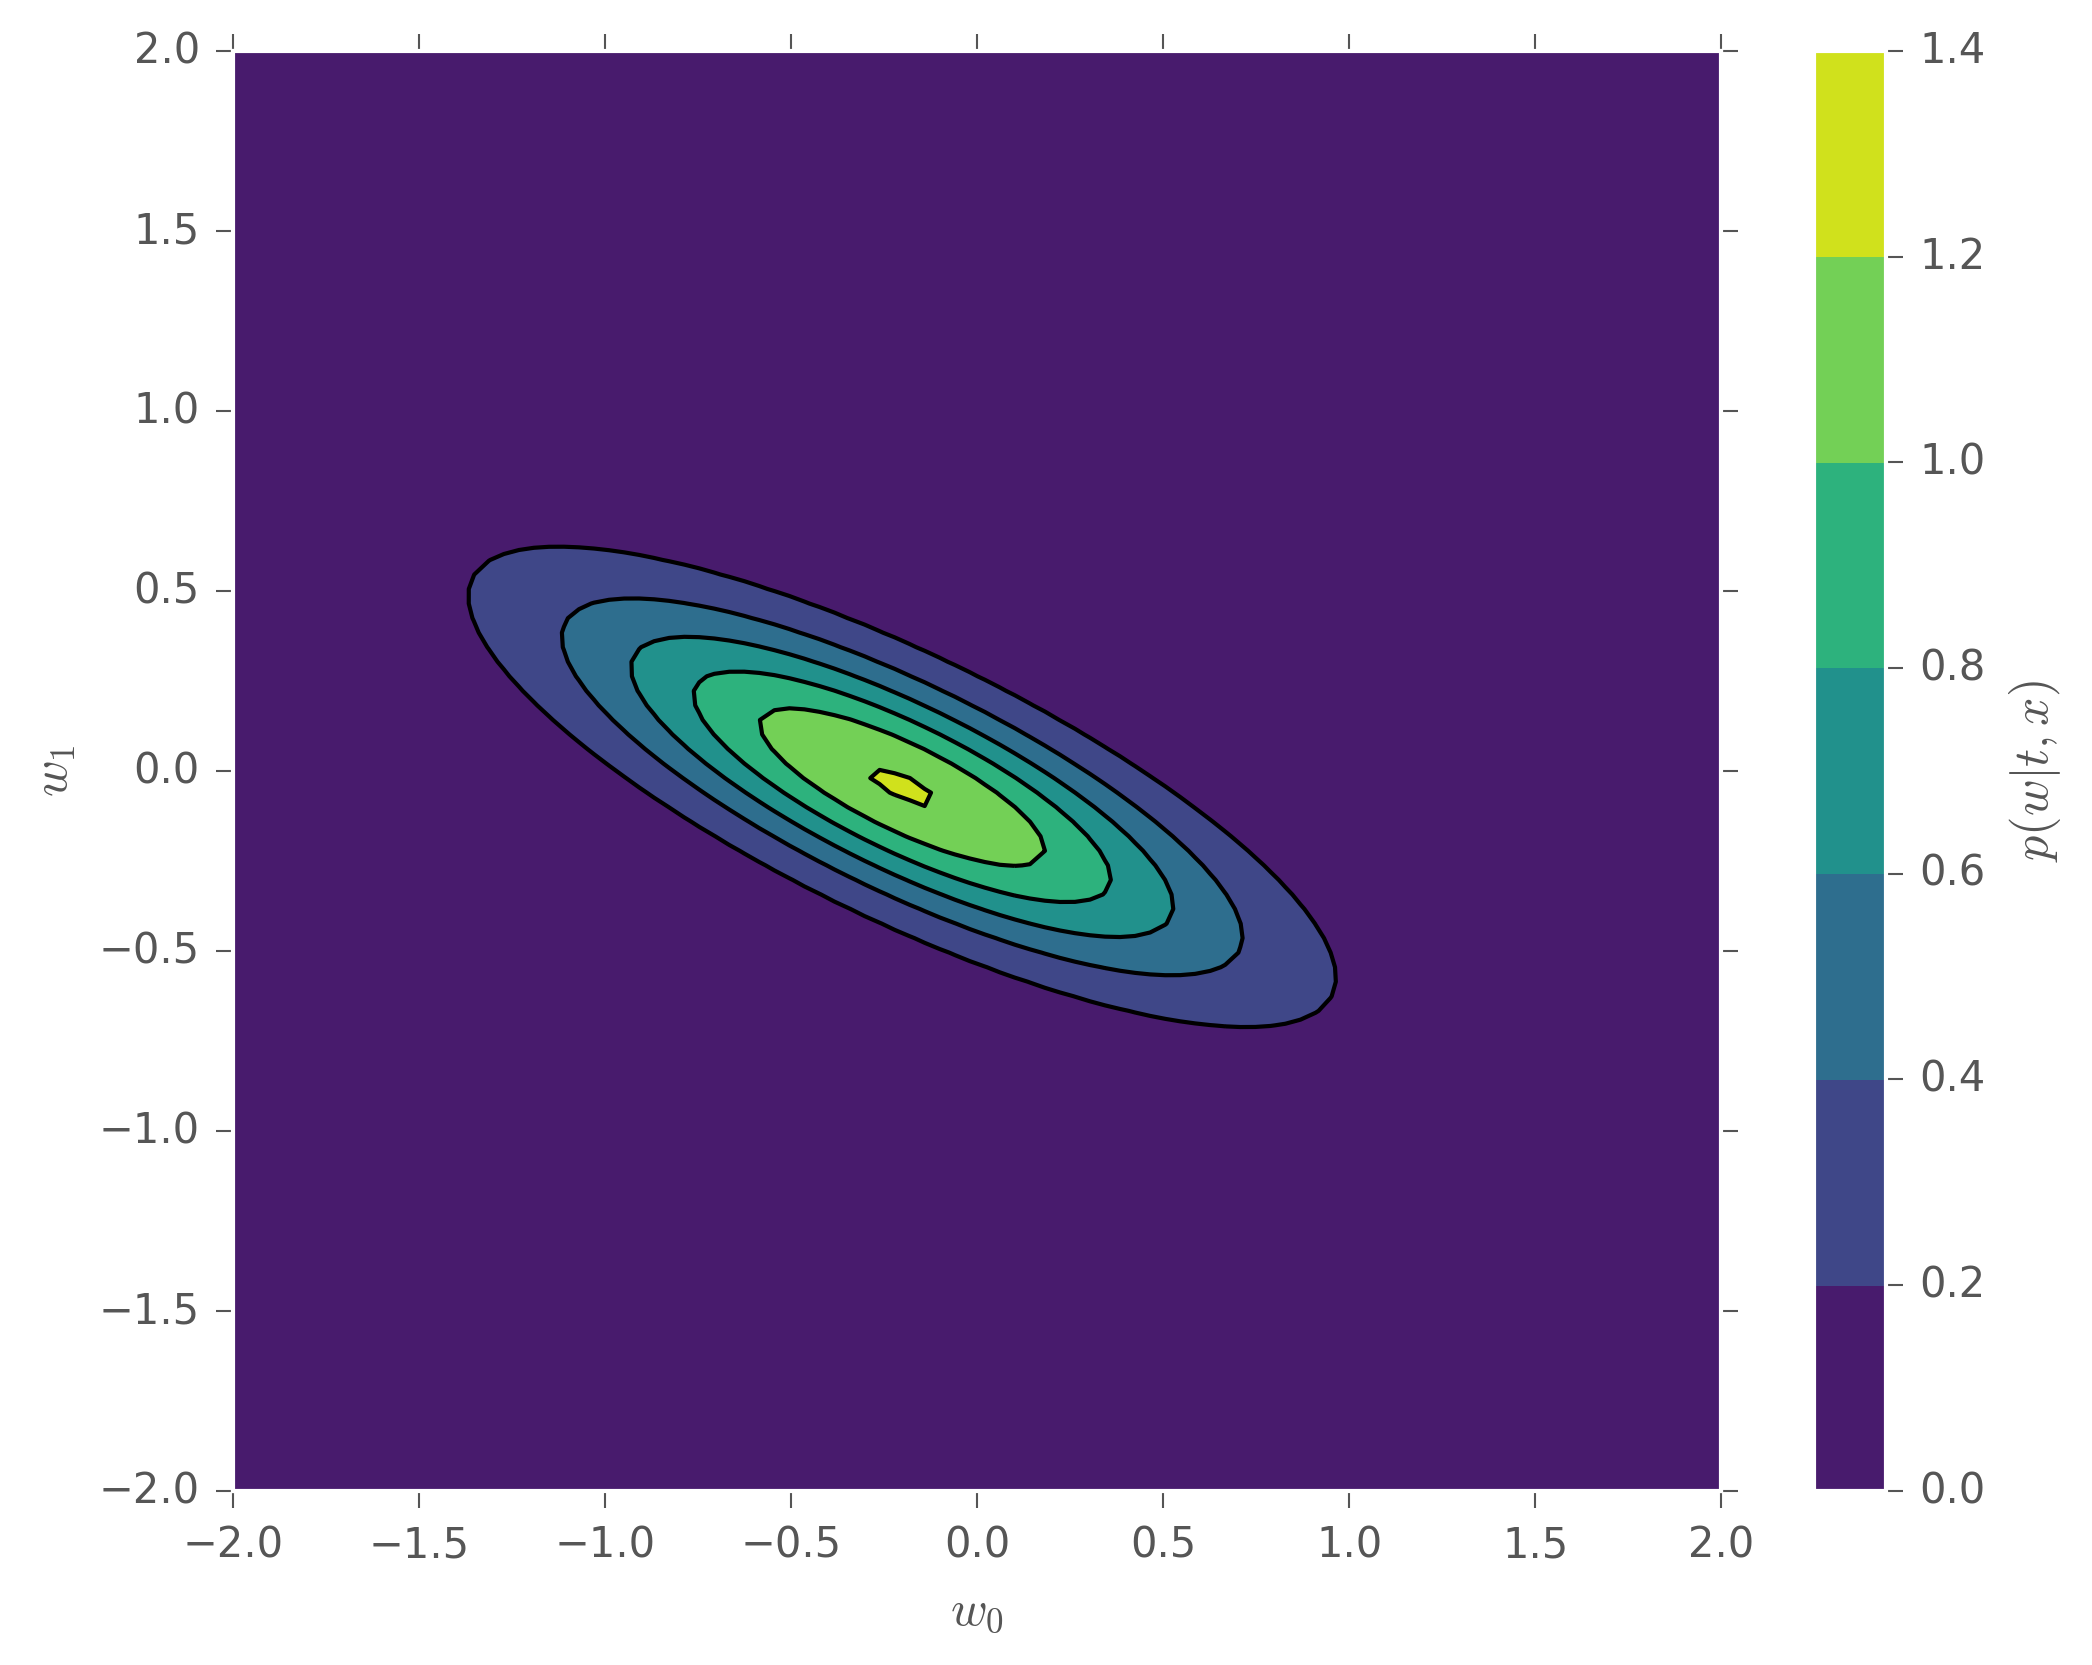
\includegraphics[width=.6\linewidth]{images/pw.png}
\caption{The probability distribution over the weights after observing two datapoints. Assuming the observed data points were not influenced by any noise, the weights should be $w_1=\frac{-0.35 - 0.05}{0.6 - 0.4}=-2$ and $t=w_0+w_1x \Rightarrow w_0=t-w_1x=0.05+2*0.4= 0.85$}
\label{fig:pw}
\end{figure}
\end{enumerate}

\section*{Exercise 2 -- Logistic Regression}
\subsection*{Part 1 -- The IRLS algorithm}
\begin{enumerate}
\item
The expression for minimizing $f(x) = \sin(x)$ using the Newton-Raphson method is
\begin{align*}
x^{(n+1)}&=x^{(n)} - \frac{f'(x^{(n)})}{f''(x^{(n)})} \\
&=x^{(n)} + \frac{\cos(x^{(n)})}{\sin(x^{(n)})}.
\end{align*}
Which translates to the following code:
\begin{lstlisting}
function nr_sin(x)
    x + cos(x)/sin(x)
end
\end{lstlisting}
For $x^{(0)}=1$, the algorithm converges to the maximum in 3 steps. For $x^{(0)}=-1$, the algorithm coverges to a minimum in 3 steps.
\item The Newton-Raphson update rule for logistic regression is
\begin{align*}
\bm{w}^{\text{(new)}}&=(\bm{\Phi}^T\bm{R}\bm{\Phi})^{-1}\bm{\Phi}^T\bm{R}\textbf{z} \\
\textbf{z}&=\bm{\Phi}\bm{w}^{\text{(old)}}-\bm{R}^{-1}(\textbf{y} - \textbf{t}).
\end{align*}
From this, we can come up with the following Julia implementation
\begin{lstlisting}
for _ in 1:5
    y = reshape(1. ./ (1+exp(-w' * phi)), N)
    R = diagm(y .* (1-y))
    z = phi' * w - inv(R) * (y - t)
    w = inv(phi*R*phi') * phi * R * z
end
\end{lstlisting}
After 4 iterations, the weights are approximately $[9.8, -21.7]\approx\hat{\bm{w}}^T$.
The decision boundary can be found by solving the following equation for $\phi$
\begin{align*}
p(C_1|\bm{\phi}) &= \frac{1}{1+e^{-\bm{w}^T\bm{\phi}}} \\
0.5 &=  \frac{1}{1+e^{-[9.8, -21.7]^T [1, \phi]}} \\
0.5 &=  \frac{1}{1+e^{-9.8 + 21.7\phi}} \\
2 &=  1+e^{-9.8 + 21.7\phi} \\
1 &=  e^{-9.8 + 21.7\phi} \\
\ln(1) &=  -9.8 + 21.7\phi \\
0 &=  -9.8 + 21.7\phi \\
21.7\phi &=  9.8 \\
\phi &= \frac{9.8}{21.7} \approx 0.45
\end{align*}
\end{enumerate}
\subsection*{Part 2 -- Two-class classification using logistic regression}
We can generate a plot with the following code:
\begin{lstlisting}
data = readdlm("a010_irlsdata.txt")
X = data[:, 1:2]
C = data[:, 3]

scatter(X[C .== 0, 1], X[C .== 0, 2], c="b", label=L"$C=0$")
scatter(X[C .== 1, 1], X[C .== 1, 2], c="r", label=L"$C=1$")
\end{lstlisting}
\begin{figure}[H]
\centering
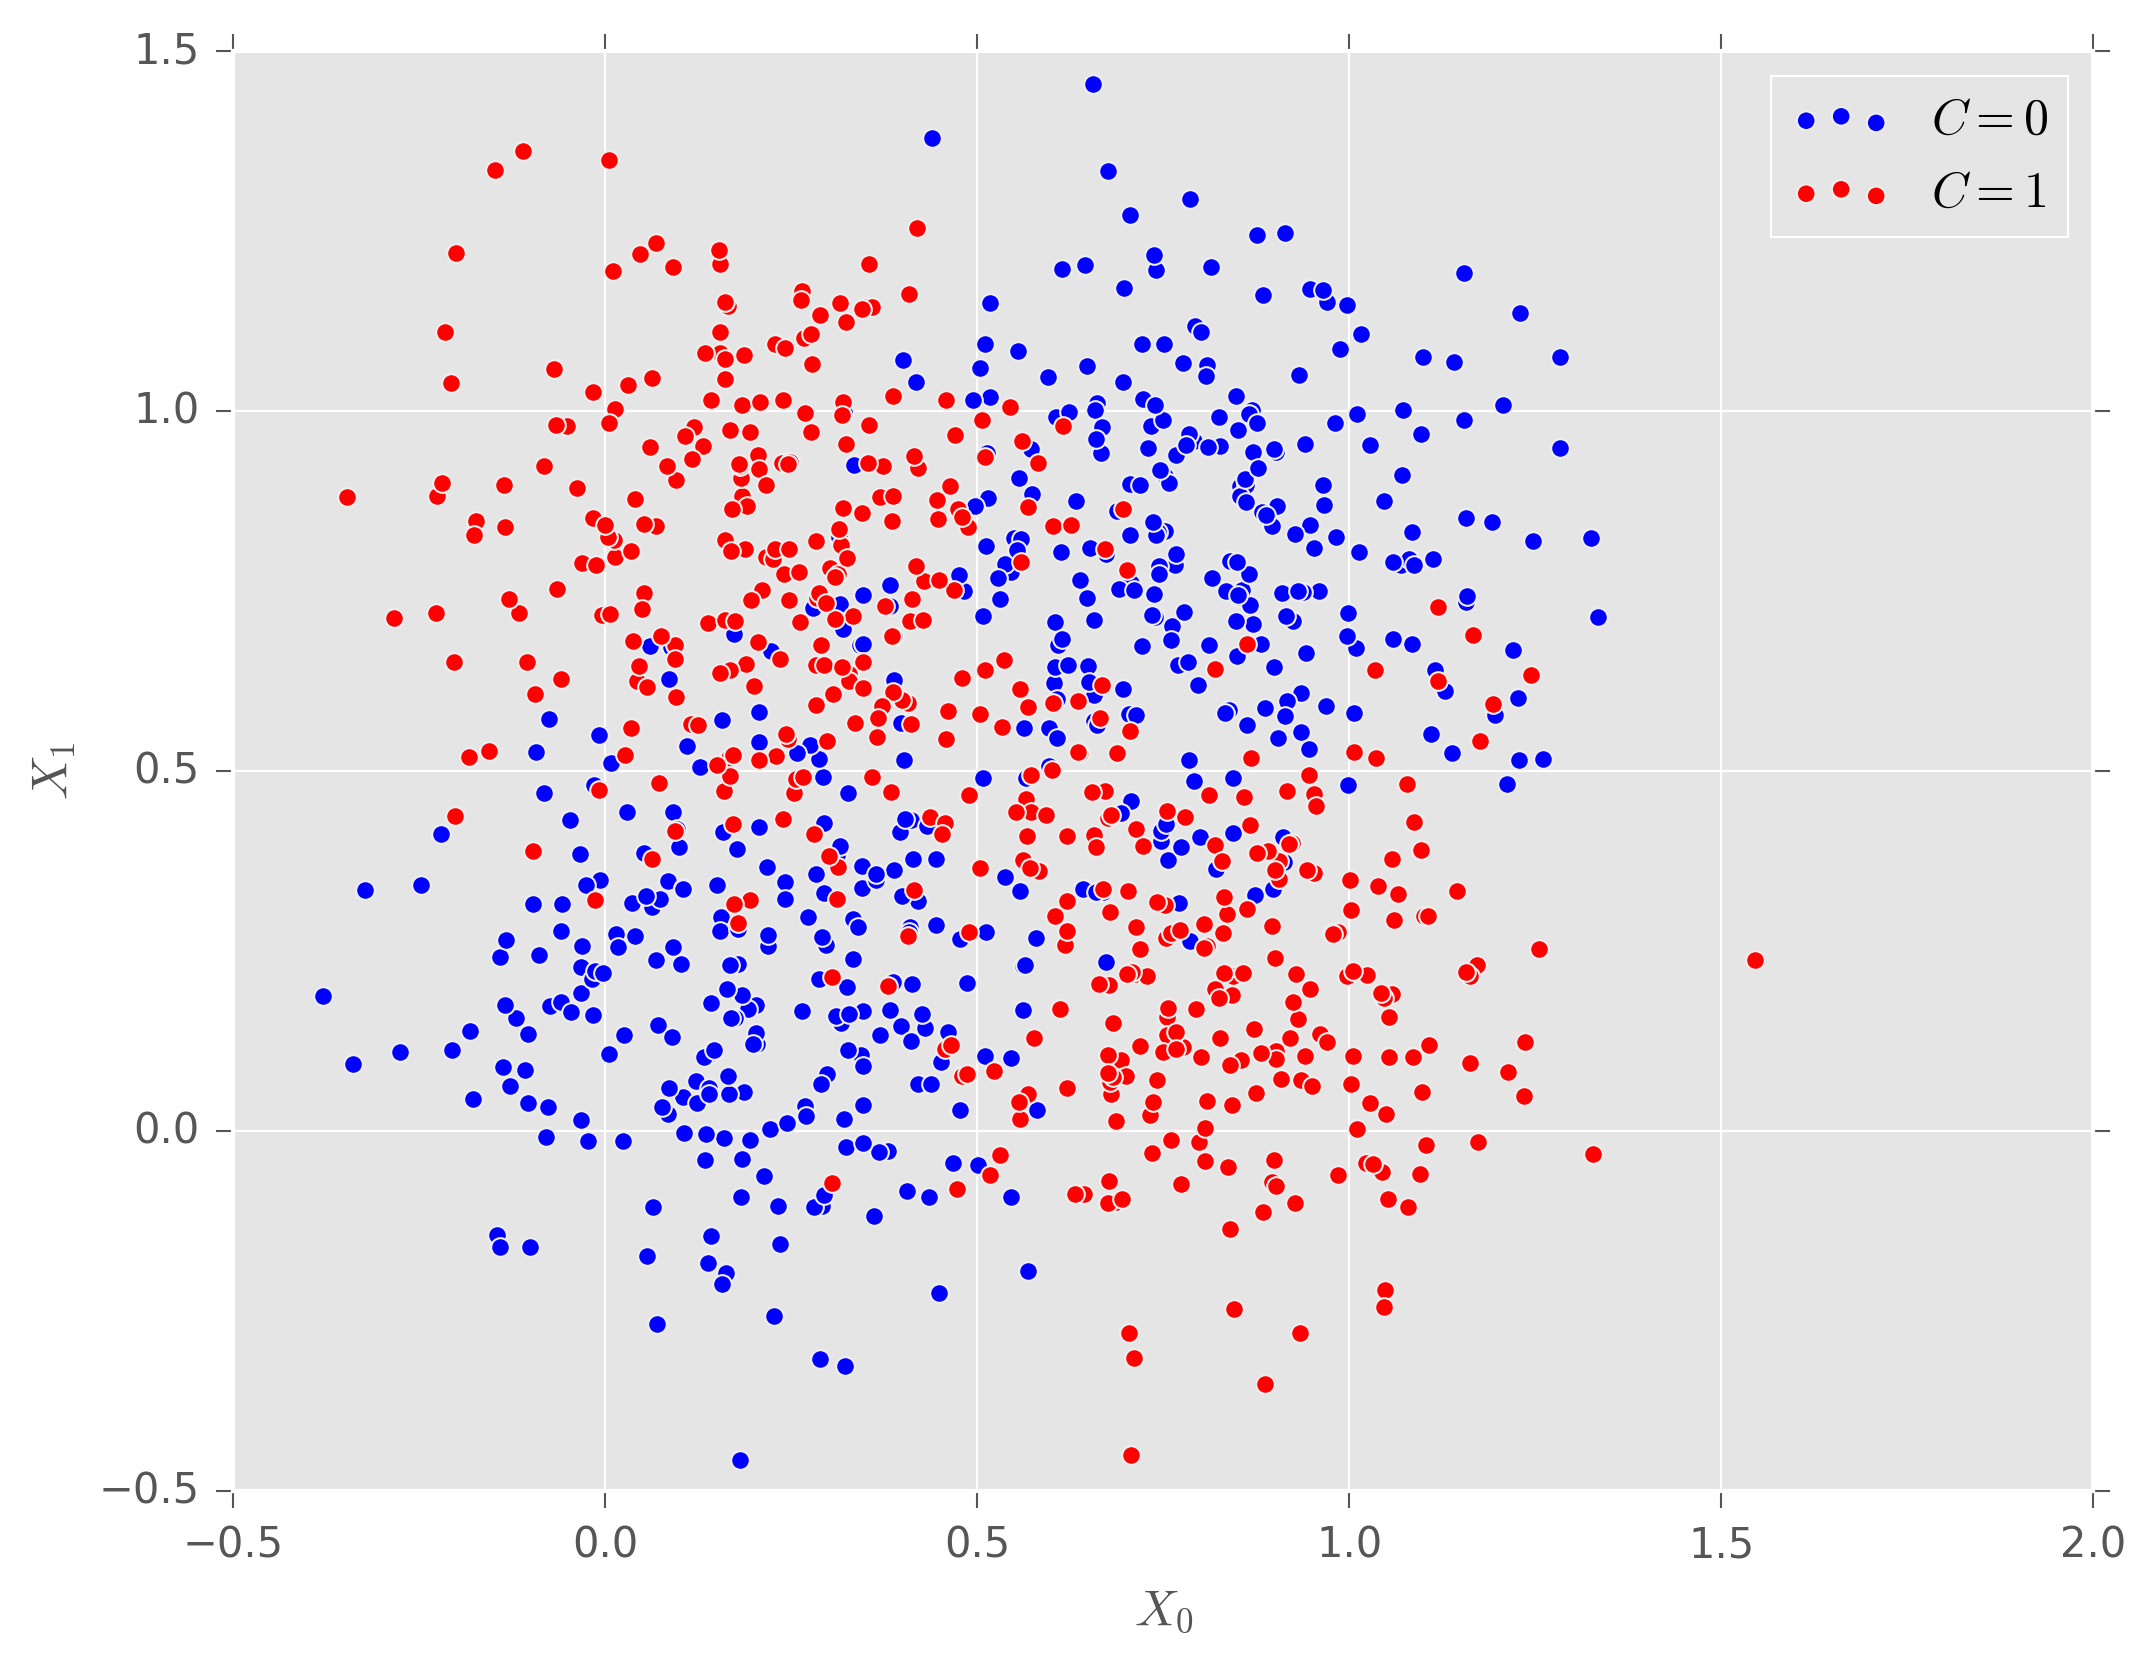
\includegraphics[width=.6\linewidth]{images/scatter.png}
\caption{A scatter plot of the two classes}
\label{fig:scatter}
\end{figure}
I think logistic regression will have difficulties classifying this data. There is a large area where the both classes are represented equally. However, there are also some areas which strictly belong to a single class.
\end{document}